\documentclass[11pt,preprint, authoryear]{elsarticle}

\usepackage{lmodern}
%%%% My spacing
\usepackage{setspace}
\setstretch{1.2}
\DeclareMathSizes{12}{14}{10}{10}

% Wrap around which gives all figures included the [H] command, or places it "here". This can be tedious to code in Rmarkdown.
\usepackage{float}
\let\origfigure\figure
\let\endorigfigure\endfigure
\renewenvironment{figure}[1][2] {
    \expandafter\origfigure\expandafter[H]
} {
    \endorigfigure
}

\let\origtable\table
\let\endorigtable\endtable
\renewenvironment{table}[1][2] {
    \expandafter\origtable\expandafter[H]
} {
    \endorigtable
}


\usepackage{ifxetex,ifluatex}
\usepackage{fixltx2e} % provides \textsubscript
\ifnum 0\ifxetex 1\fi\ifluatex 1\fi=0 % if pdftex
  \usepackage[T1]{fontenc}
  \usepackage[utf8]{inputenc}
\else % if luatex or xelatex
  \ifxetex
    \usepackage{mathspec}
    \usepackage{xltxtra,xunicode}
  \else
    \usepackage{fontspec}
  \fi
  \defaultfontfeatures{Mapping=tex-text,Scale=MatchLowercase}
  \newcommand{\euro}{€}
\fi

\usepackage{amssymb, amsmath, amsthm, amsfonts}

\def\bibsection{\section*{References}} %%% Make "References" appear before bibliography


\usepackage[round]{natbib}

\usepackage{longtable}
\usepackage[margin=2.3cm,bottom=2cm,top=2.5cm, includefoot]{geometry}
\usepackage{fancyhdr}
\usepackage[bottom, hang, flushmargin]{footmisc}
\usepackage{graphicx}
\numberwithin{equation}{section}
\numberwithin{figure}{section}
\numberwithin{table}{section}
\setlength{\parindent}{0cm}
\setlength{\parskip}{1.3ex plus 0.5ex minus 0.3ex}
\usepackage{textcomp}
\renewcommand{\headrulewidth}{0.2pt}
\renewcommand{\footrulewidth}{0.3pt}

\usepackage{array}
\newcolumntype{x}[1]{>{\centering\arraybackslash\hspace{0pt}}p{#1}}

%%%%  Remove the "preprint submitted to" part. Don't worry about this either, it just looks better without it:
\makeatletter
\def\ps@pprintTitle{%
  \let\@oddhead\@empty
  \let\@evenhead\@empty
  \let\@oddfoot\@empty
  \let\@evenfoot\@oddfoot
}
\makeatother

 \def\tightlist{} % This allows for subbullets!

\usepackage{hyperref}
\hypersetup{breaklinks=true,
            bookmarks=true,
            colorlinks=true,
            citecolor=blue,
            urlcolor=blue,
            linkcolor=blue,
            pdfborder={0 0 0}}


% The following packages allow huxtable to work:
\usepackage{siunitx}
\usepackage{multirow}
\usepackage{hhline}
\usepackage{calc}
\usepackage{tabularx}
\usepackage{booktabs}
\usepackage{caption}


\newenvironment{columns}[1][]{}{}

\newenvironment{column}[1]{\begin{minipage}{#1}\ignorespaces}{%
\end{minipage}
\ifhmode\unskip\fi
\aftergroup\useignorespacesandallpars}

\def\useignorespacesandallpars#1\ignorespaces\fi{%
#1\fi\ignorespacesandallpars}

\makeatletter
\def\ignorespacesandallpars{%
  \@ifnextchar\par
    {\expandafter\ignorespacesandallpars\@gobble}%
    {}%
}
\makeatother

\newenvironment{CSLReferences}[2]{%
}

\urlstyle{same}  % don't use monospace font for urls
\setlength{\parindent}{0pt}
\setlength{\parskip}{6pt plus 2pt minus 1pt}
\setlength{\emergencystretch}{3em}  % prevent overfull lines
\setcounter{secnumdepth}{5}

%%% Use protect on footnotes to avoid problems with footnotes in titles
\let\rmarkdownfootnote\footnote%
\def\footnote{\protect\rmarkdownfootnote}
\IfFileExists{upquote.sty}{\usepackage{upquote}}{}

%%% Include extra packages specified by user
\usepackage{booktabs}
\usepackage{longtable}
\usepackage{array}
\usepackage{multirow}
\usepackage{wrapfig}
\usepackage{float}
\usepackage{colortbl}
\usepackage{pdflscape}
\usepackage{tabu}
\usepackage{threeparttable}
\usepackage{threeparttablex}
\usepackage[normalem]{ulem}
\usepackage{makecell}
\usepackage{xcolor}

%%% Hard setting column skips for reports - this ensures greater consistency and control over the length settings in the document.
%% page layout
%% paragraphs
\setlength{\baselineskip}{12pt plus 0pt minus 0pt}
\setlength{\parskip}{12pt plus 0pt minus 0pt}
\setlength{\parindent}{0pt plus 0pt minus 0pt}
%% floats
\setlength{\floatsep}{12pt plus 0 pt minus 0pt}
\setlength{\textfloatsep}{20pt plus 0pt minus 0pt}
\setlength{\intextsep}{14pt plus 0pt minus 0pt}
\setlength{\dbltextfloatsep}{20pt plus 0pt minus 0pt}
\setlength{\dblfloatsep}{14pt plus 0pt minus 0pt}
%% maths
\setlength{\abovedisplayskip}{12pt plus 0pt minus 0pt}
\setlength{\belowdisplayskip}{12pt plus 0pt minus 0pt}
%% lists
\setlength{\topsep}{10pt plus 0pt minus 0pt}
\setlength{\partopsep}{3pt plus 0pt minus 0pt}
\setlength{\itemsep}{5pt plus 0pt minus 0pt}
\setlength{\labelsep}{8mm plus 0mm minus 0mm}
\setlength{\parsep}{\the\parskip}
\setlength{\listparindent}{\the\parindent}
%% verbatim
\setlength{\fboxsep}{5pt plus 0pt minus 0pt}



\begin{document}



\begin{frontmatter}  %

\title{Predicting Employee Attrition}

% Set to FALSE if wanting to remove title (for submission)




\author[Add1]{Hannah MacGinty}
\ead{21082022@sun.ac.za}





\address[Add1]{Stellenbosch University, South Africa}

\cortext[cor]{Corresponding author: Hannah MacGinty}

\begin{abstract}
\small{
This paper investigates employee attributes and attrition. Random
forests are used to build a model to predict employee attrition based on
key attributes, such as education, pay, gender, and age, among others.
}
\end{abstract}

\vspace{1cm}





\vspace{0.5cm}

\end{frontmatter}

\setcounter{footnote}{0}



%________________________
% Header and Footers
%%%%%%%%%%%%%%%%%%%%%%%%%%%%%%%%%
\pagestyle{fancy}
\chead{}
\rhead{}
\lfoot{}
\rfoot{\footnotesize Page \thepage}
\lhead{}
%\rfoot{\footnotesize Page \thepage } % "e.g. Page 2"
\cfoot{}

%\setlength\headheight{30pt}
%%%%%%%%%%%%%%%%%%%%%%%%%%%%%%%%%
%________________________

\headsep 35pt % So that header does not go over title




\hypertarget{introduction}{%
\section{\texorpdfstring{Introduction
\label{Introduction}}{Introduction }}\label{introduction}}

Losing employees can be costly for businesses. Predicting attrition and
its key determinants or attributes can help estimate future employee
turnover and attempt to reduce it.

\hypertarget{exploratory-data-analaysis}{%
\section*{Exploratory Data Analaysis}\label{exploratory-data-analaysis}}
\addcontentsline{toc}{section}{Exploratory Data Analaysis}

The dataset contains information on 4653 employees and whether they
attrited or not. The employee attributes available include demographic
information such as age and gender. Employees are based in one of three
major cities in India, namely Bangalore, Pune and New Delhi. The year an
employee joined a company (Joining Year), ranging from 2014 to 2018, is
also considered.

Given that earnings are generally an important determinant in whether an
employee leaves their job, their payment tier, scaled from 1, being the
highest, and 3, being the lowest, is included in the data. Additionally,
years of experience in their current field is included as well as their
highest level of education (Bachelor's, Master's, PhD). There is also
information on whether an employee kept out of projects for 1 month or
more, which could potentially indicates an employee's lack of interest
in work or plans to leave the company.

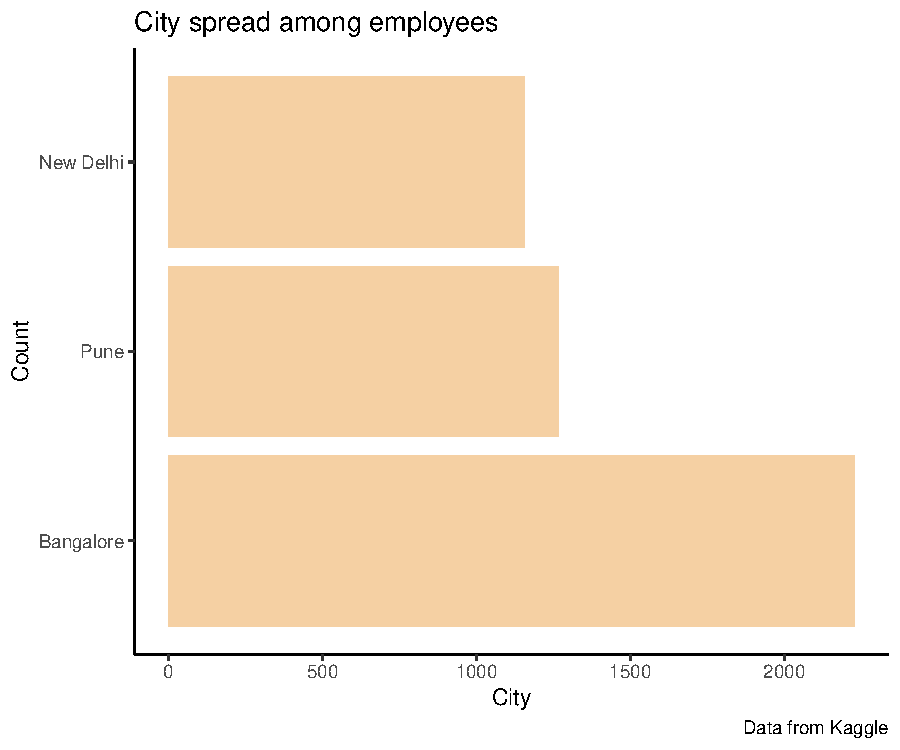
\includegraphics{Final_project_files/figure-latex/unnamed-chunk-2-1.pdf}

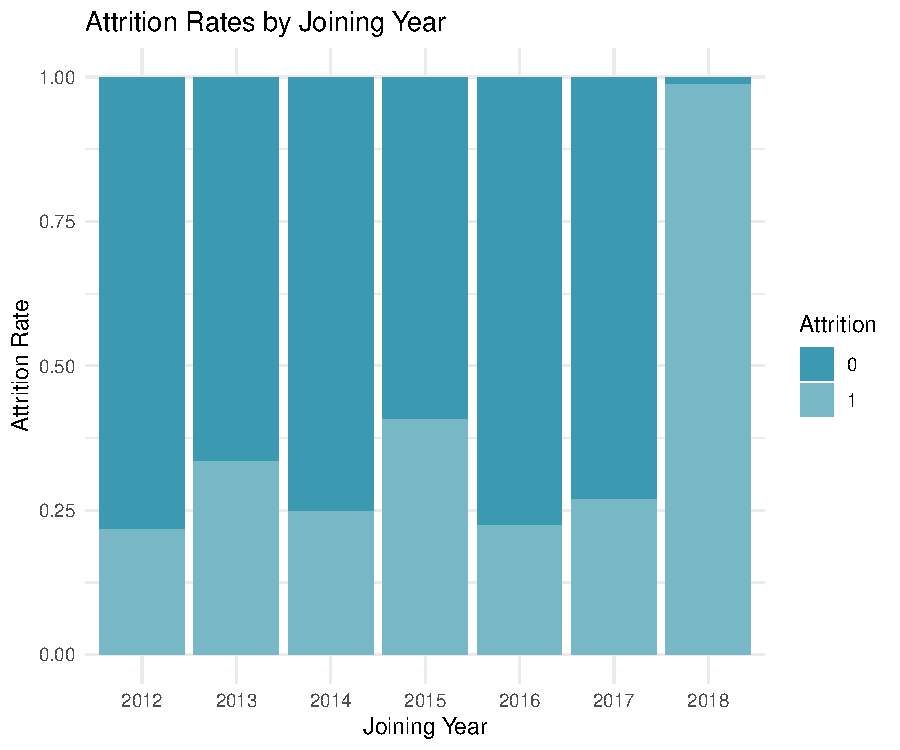
\includegraphics{Final_project_files/figure-latex/unnamed-chunk-3-1.pdf}

Spreading the data among city, most of the employees are from Bangalore.
Additionally, most employees have a Bachelors degree. Only 179 employees
have a PHD and 873 have Master's degrees. Looking at age, which ranges
between 22 and 41, the majority of employees are in their mid to late
twenties, skewing the distribution to right.

Regarding experience, very few individuals have 6 or 7 years experience
(only 16 employees in total) in their current field of work, most likely
due to the young employee base. Most commonly, individuals have 2 years
experience.

2017 saw the most employees join the company. There was a substantial
fall in employees joining in 2018. Only 367 employees joined in 2018,
compared to 1180 in 2017.

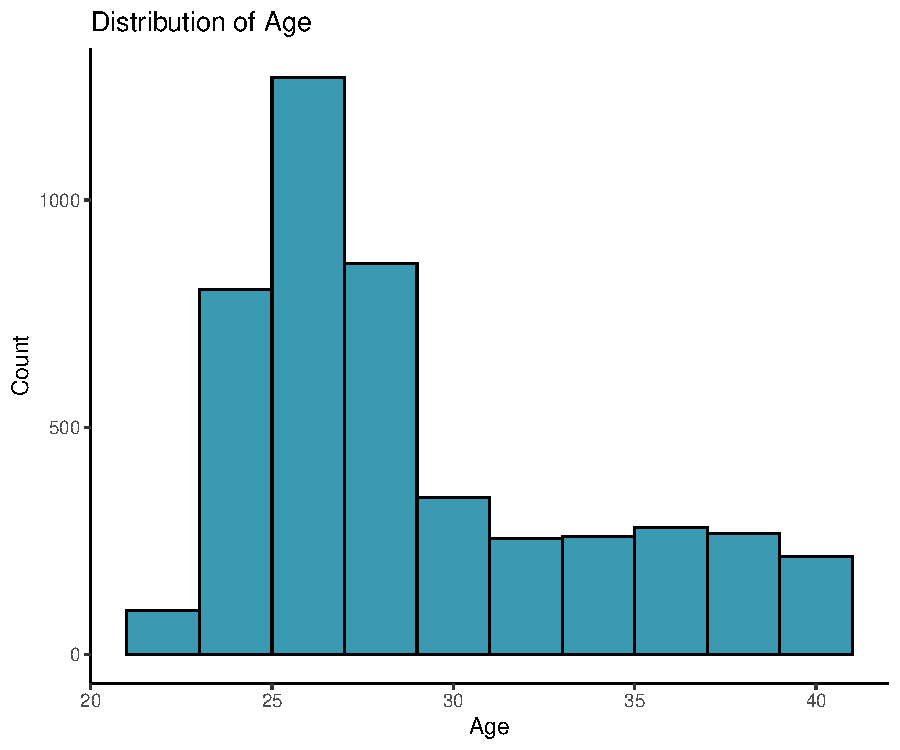
\includegraphics{Final_project_files/figure-latex/unnamed-chunk-4-1.pdf}

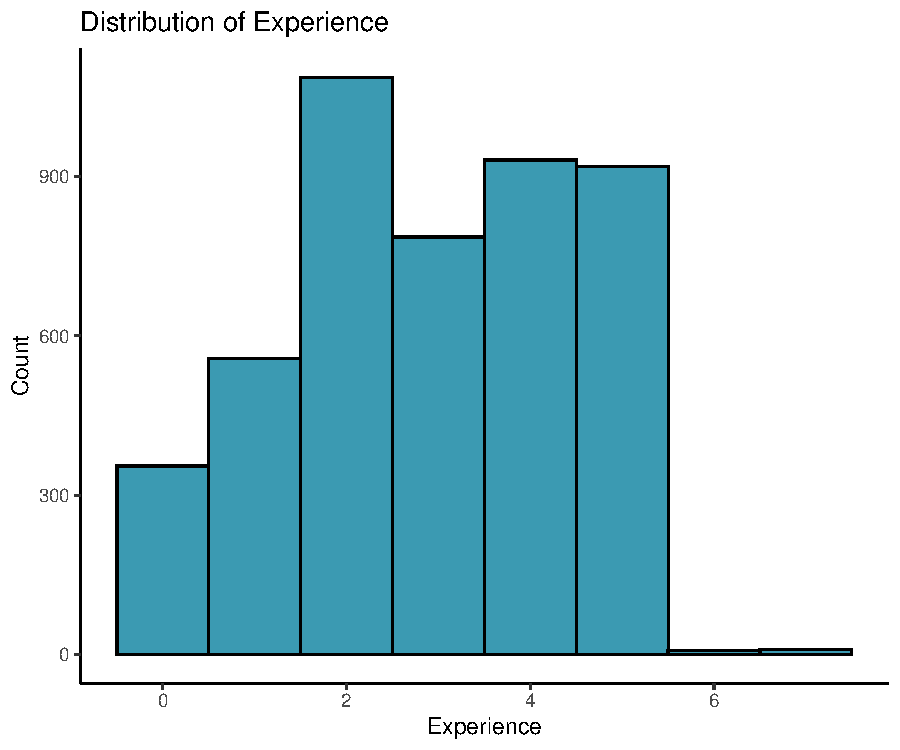
\includegraphics{Final_project_files/figure-latex/unnamed-chunk-5-1.pdf}

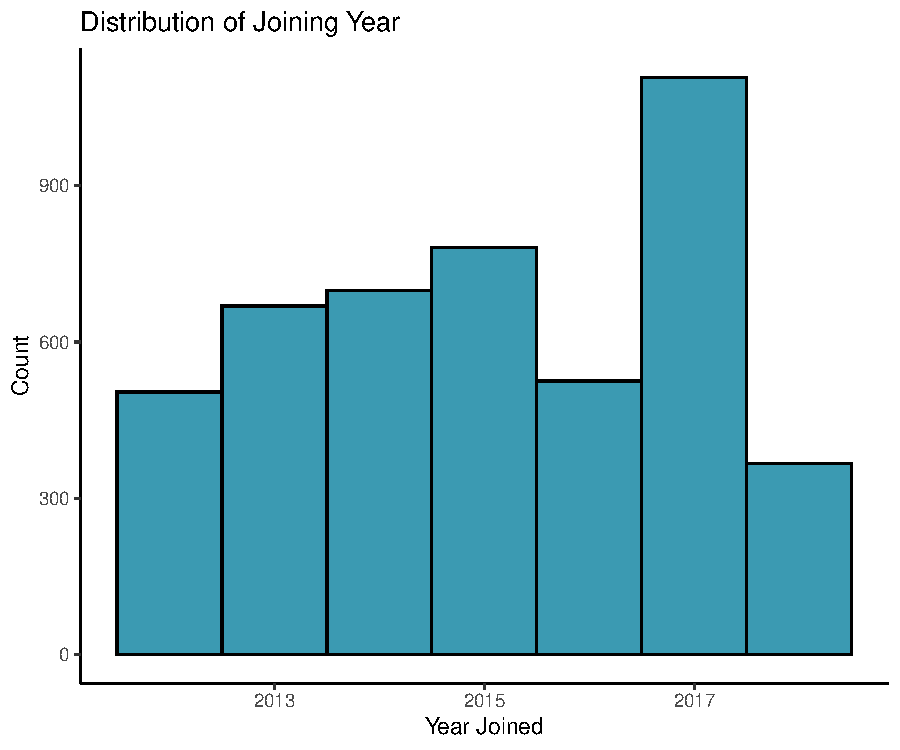
\includegraphics{Final_project_files/figure-latex/unnamed-chunk-6-1.pdf}

Attrition rates are highest among those with Master's degrees. Nearly
fifty percent of those with Master's degrees left their job. When
looking across joining year, almost all the employees that joined in
2018 resigned. It is possible that some event occurred in 2018 that
caused that cohort to leave within the next two years.

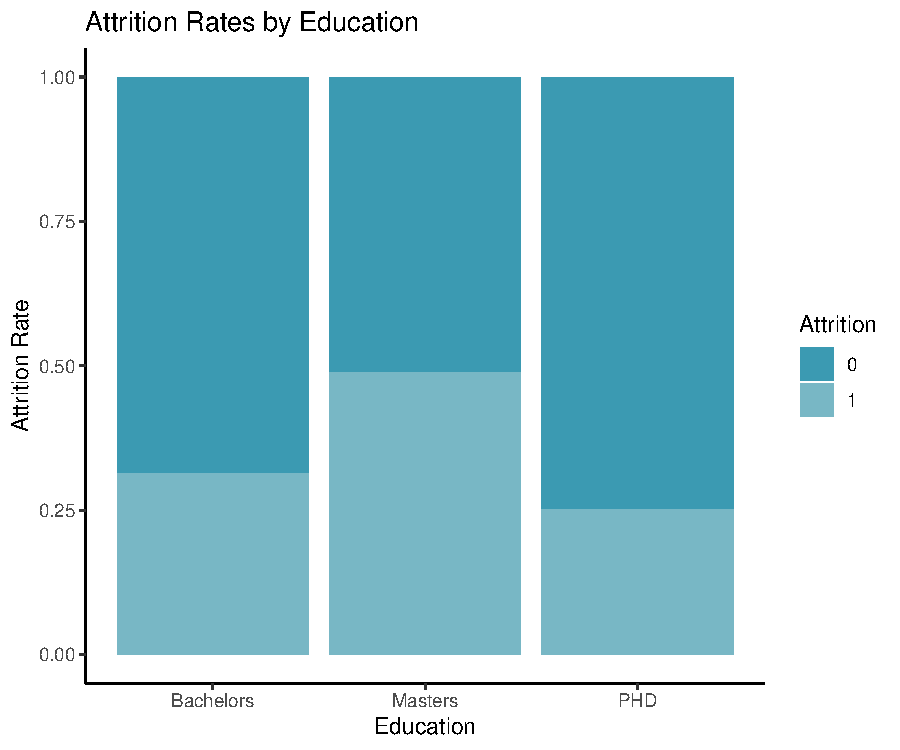
\includegraphics{Final_project_files/figure-latex/unnamed-chunk-7-1.pdf}

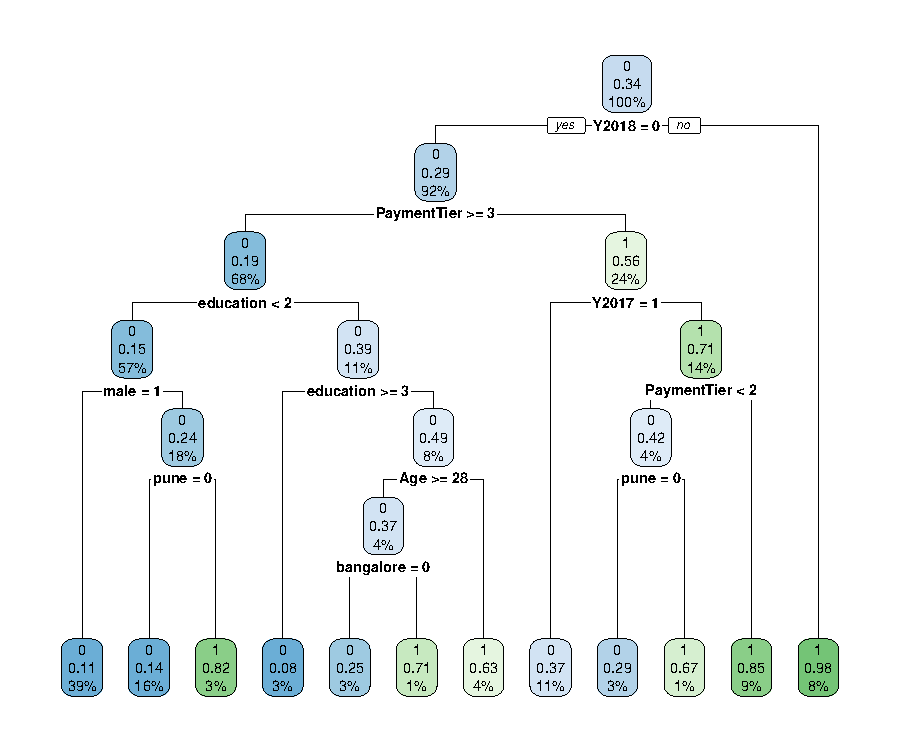
\includegraphics{Final_project_files/figure-latex/unnamed-chunk-8-1.pdf}

The table below presents the attrition rate across education, gender,
city, joining year, experience, and pay level. Attrition rates are
particularly high for individuals who joined in 2018 (98\%), matching
the graphical analysis. It is also high for those earning a mid-tier
salary (almost 60\%). This is followed by 50\% of those from Pune
attriting.

\begin{table}[H]
\centering
\begin{tabular}{rllr}
  \hline
 & Variable & Category & Attrition.Rate \\ 
  \hline
1 & Education & Bachelors & 31.35 \\ 
  2 & Education & Masters & 48.80 \\ 
  3 & Education & PHD & 25.14 \\ 
  4 & City & Bangalore & 26.71 \\ 
  5 & City & New Delhi & 31.63 \\ 
  6 & City & Pune & 50.39 \\ 
  7 & Gender & Female & 47.15 \\ 
  8 & Gender & Male & 25.77 \\ 
  9 & Year & 2012 & 21.63 \\ 
  10 & Year & 2013 & 33.48 \\ 
  11 & Year & 2014 & 24.75 \\ 
  12 & Year & 2015 & 40.72 \\ 
  13 & Year & 2016 & 22.29 \\ 
  14 & Year & 2017 & 26.81 \\ 
  15 & Year & 2018 & 98.64 \\ 
  16 & Pay & 1 & 36.63 \\ 
  17 & Pay & 2 & 59.91 \\ 
  18 & Pay & 3 & 27.52 \\ 
   \hline
\end{tabular}
\caption{Attrition Rate Across Categories \label{tab1}} 
\end{table}

\hypertarget{feature-and-target-engineering}{%
\section*{Feature and Target
Engineering}\label{feature-and-target-engineering}}
\addcontentsline{toc}{section}{Feature and Target Engineering}

Since my predictor variable (Leave or Not) is binary, there is no need
for target engineering.

Regarding feature engineering, most of the features are categorical.
Gender and whether a person benched or not (removed themselves from
projects in the lst month) are transformed into dummies. Joining year is
one-hot encoded, resulting in binary variables for each of the 5 joining
years.

Education is label encoded as it can be ordered (Bachelors being the
lowest level of education, Master's one higher and PHD being the highest
level of education). Payment Tier and experience in the current domain
were already label encoded and thus do not require further engineering.

Since age is numeric and random forests are able to handle both numeric
and categorical variables, it is not altered.

\hypertarget{logistic-regression}{%
\section*{Logistic Regression}\label{logistic-regression}}
\addcontentsline{toc}{section}{Logistic Regression}

Logistic regression is often used for binary classification problems.

Using logistic regression, three models are estimated to assess the
accuracy of predicting employee attrition. Model 1 regresses employee
attrition on education level. Model 2 adds payment tier as another
feature. Model 3 regresses employee attrition on all available features.

\begin{table}[H]
\centering
\begin{tabular}{rrrrrrrr}
  \hline
 & Min. & 1st Qu. & Median & Mean & 3rd Qu. & Max. & NA's \\ 
  \hline
1 & 0.63 & 0.64 & 0.65 & 0.64 & 0.66 & 0.66 & 0.00 \\ 
  2 & 0.60 & 0.62 & 0.63 & 0.63 & 0.65 & 0.66 & 0.00 \\ 
  3 & 0.70 & 0.72 & 0.74 & 0.74 & 0.75 & 0.76 & 0.00 \\ 
   \hline
\end{tabular}
\caption{Accuracy across logistic models \label{tab1}} 
\end{table}

From the logistic regression, model accuracy ranges from 70 and 76
percent for the full model. The weakest model is model 1, which
regresses attrition on education, has an accuracy rate between 63 and 66
percent.

In terms of the most important features, gender and the joining year of
2017 are the most important predictive features. Most of the other
variables do carry some level of importance, therefore the model is not
overly reliant on gender and joining year. This also provides an
indication that the variance of the model is not too high. While the
model suffers some level of bias, given that the accuracy is the model
is approximately 74 percent, it does not suffer from high bias.

\begin{table}[H]
\centering
\begin{tabular}{rlll}
  \hline
 & Reference & Prediction & Count \\ 
  \hline
1 & 1 & 1 &  483 \\ 
  2 & 1 & 0 &  637 \\ 
  3 & 0 & 1 &  204 \\ 
  4 & 0 & 0 & 1933 \\ 
   \hline
\end{tabular}
\caption{Confusion Matrix for Logistic Model \label{tab1}} 
\end{table}

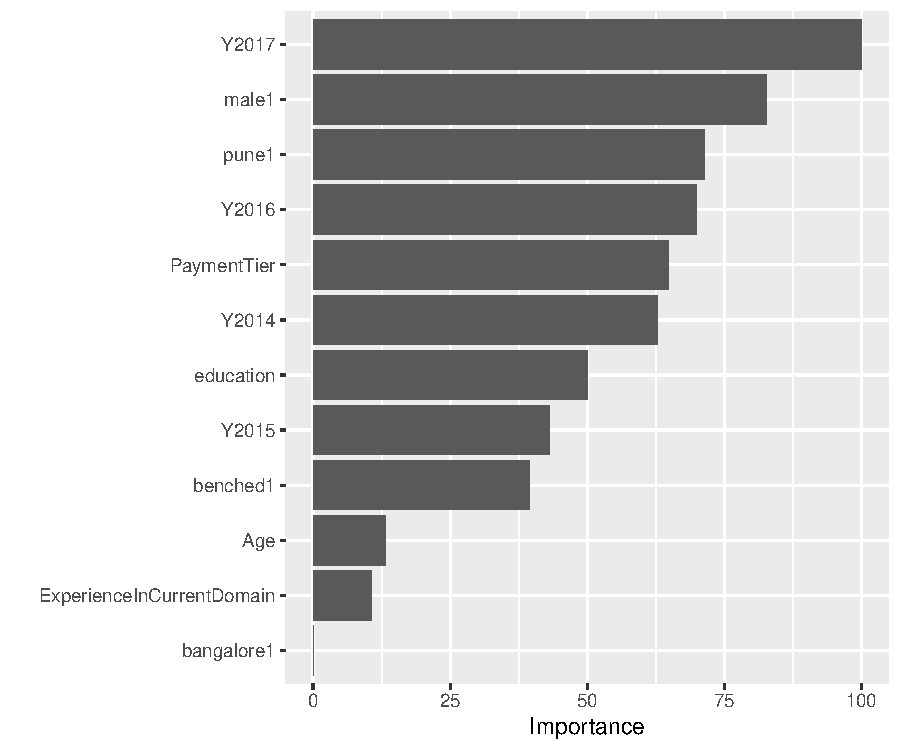
\includegraphics{Final_project_files/figure-latex/Table2-1.pdf}

\begin{table}[H]
\centering
\begin{tabular}{rlr}
  \hline
 & Metric & Value \\ 
  \hline
1 & Accuracy & 0.74 \\ 
  2 & F1 Score & 0.53 \\ 
  3 & Recall & 0.43 \\ 
  4 & Precision & 0.70 \\ 
   \hline
\end{tabular}
\caption{Metrics for Logistic Regression \label{tab1}} 
\end{table}

\begin{table}[H]
\centering
\begin{tabular}{rlr}
  \hline
 & Metric & Value \\ 
  \hline
1 & Training Accuracy & 0.74 \\ 
  2 & Test Accuracy & 0.71 \\ 
  3 & Training Error & 0.26 \\ 
  4 & Test Error & 0.29 \\ 
   \hline
\end{tabular}
\caption{More Metrics for Logistic Regression \label{tab1}} 
\end{table}

\begin{table}[H]
\centering
\begin{tabular}{rlrrrr}
  \hline
 & term & estimate & std.error & statistic & p.value \\ 
  \hline
1 & (Intercept) & 1.86 & 0.39 & 4.79 & 0.00 \\ 
  2 & Age & -0.02 & 0.01 & -2.73 & 0.01 \\ 
  3 & male1 & -0.81 & 0.09 & -9.48 & 0.00 \\ 
  4 & benched1 & 0.67 & 0.13 & 5.29 & 0.00 \\ 
  5 & ExperienceInCurrentDomain & -0.07 & 0.03 & -2.48 & 0.01 \\ 
  6 & bangalore1 & 0.17 & 0.12 & 1.45 & 0.15 \\ 
  7 & pune1 & 0.99 & 0.12 & 8.38 & 0.00 \\ 
  8 & education & 0.53 & 0.08 & 6.31 & 0.00 \\ 
  9 & PaymentTier & -0.60 & 0.08 & -7.75 & 0.00 \\ 
  10 & Y2014 & -0.97 & 0.13 & -7.56 & 0.00 \\ 
  11 & Y2015 & -0.69 & 0.12 & -5.63 & 0.00 \\ 
  12 & Y2016 & -1.23 & 0.15 & -8.23 & 0.00 \\ 
  13 & Y2017 & -1.30 & 0.12 & -11.16 & 0.00 \\ 
   \hline
\end{tabular}
\caption{Logistic Regression Results \label{tab1}} 
\end{table}

\hypertarget{knn}{%
\section*{KNN}\label{knn}}
\addcontentsline{toc}{section}{KNN}

The K-nearest neighbour (KNN) algorithm predicts each observation based
on its similarity to other observations. It identifies ``k''
observations that are most similar .. and uses the most common class of
those k observations as the predicted output ().

Using the KNN approach, a grid-search is conducted to find the optimal
level of K. Low values of K makes the model sensitive to noise and less
generalisable while large values can lead to oversmoothing.

The accuracy metric is used, given that is an appropriate metric for a
classification problem. The grid search uses cross-validation techniques
to looks for the optimal level of K between 2 and 25. The model selects
k =3 as the optimal value. The accuracy rate for k=3 is 78.3\%. For the
testing data, the model's accuracy is slightly lower at 77\%.

Alongside the model's accuracy, the precision, recall and F1 score are
also examined. Precision measures the proportion of correctly predicted
positive instances, also called true positives, out of all instances
predicted as positive. A high precision indicates few false positives.
In this case the precision is 74\%, which is relatively high.

Recall, also known as the model's sensitivity, measures the proportion
of correctly predicted positive instances out of all actual positives
instances. In other words, it is the proportion of true positives out of
both the true positives and false negatives. A higher recall indicates
few false negatives. In this instance, the recall is much lower (52\%).
This indicates that the model has a higher false negative rate than
false positive rate.

The F1 score balances both the precision and recall, and provides an
indication of the overall performance of the model. The F1 score for the
optimal K-nearest neighbours model is 61.2\%, indicating that the model
is somewhat adequate.

\begin{table}[H]
\centering
\begin{tabular}{rlll}
  \hline
 & Reference & Prediction & Count \\ 
  \hline
1 & 1 & 1 & 250 \\ 
  2 & 1 & 0 & 230 \\ 
  3 & 0 & 1 &  86 \\ 
  4 & 0 & 0 & 830 \\ 
   \hline
\end{tabular}
\caption{Confusion Matrix for KNN Model \label{tab1}} 
\end{table}

\begin{table}[H]
\centering
\begin{tabular}{rlr}
  \hline
 & Metric & Value \\ 
  \hline
1 & Accuracy & 0.77 \\ 
  2 & F1 Score & 0.62 \\ 
  3 & Recall & 0.53 \\ 
  4 & Precision & 0.74 \\ 
   \hline
\end{tabular}
\caption{Metrics for KNN Model \label{tab1}} 
\end{table}

\begin{table}[H]
\centering
\begin{tabular}{rlr}
  \hline
 & Metric & Value \\ 
  \hline
1 & Training Accuracy & 0.84 \\ 
  2 & Test Accuracy & 0.77 \\ 
  3 & Training Error & 0.16 \\ 
  4 & Test Error & 0.23 \\ 
   \hline
\end{tabular}
\caption{More Metrics for KNN Model \label{tab1}} 
\end{table}

\begin{table}[H]
\centering
\begin{tabular}{rlr}
  \hline
 & Metric & Value \\ 
  \hline
1 & Accuracy & 0.77 \\ 
  2 & F1 Score & 0.62 \\ 
  3 & Recall & 0.53 \\ 
  4 & Precision & 0.74 \\ 
   \hline
\end{tabular}
\caption{Metrics for KNN \label{tab1}} 
\end{table}

KNN models are very sensitive to feature scaling. Results can easily
become biased as variables with larger scales can dominate the distance
to calculation.

On the other hand, KNN is appropriate for small datasets such as this
one.

\hypertarget{random-forests}{%
\section*{Random Forests}\label{random-forests}}
\addcontentsline{toc}{section}{Random Forests}

Random forests are powerful out-of the box algorithms that generally
have very good predictive accuracy (). The come with the benefits of
decision trees and bagging but greatly reduce instability and
between-tree correlation.

\hypertarget{decision-tree}{%
\subsection*{Decision tree}\label{decision-tree}}
\addcontentsline{toc}{subsection}{Decision tree}

Following the general rule-of-thumb, there is a 70:30 split among the
training and testing data.

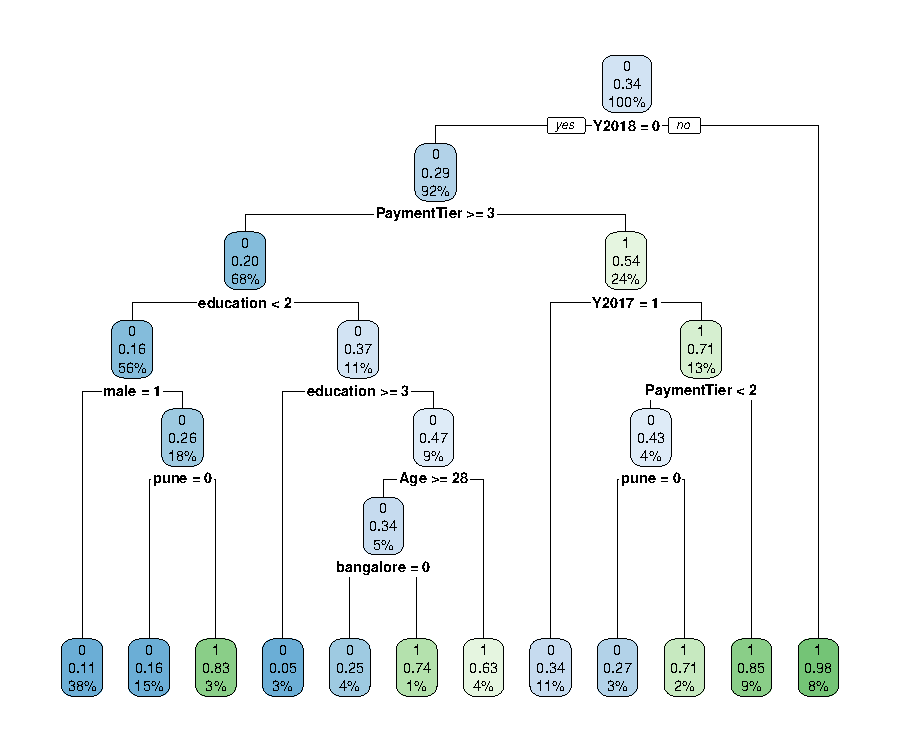
\includegraphics{Final_project_files/figure-latex/unnamed-chunk-11-1.pdf}

\hypertarget{baseline-random-forest}{%
\subsection{Baseline Random Forest}\label{baseline-random-forest}}

The results from the baseline random forest are presented below. Random
Forests help to reduce tree correlation. It does so by using
split-variable randomisation. In the baseline model, number of trees are
set to 500 by default. It is possible to alter the m(try) parameter, but
currently it is set to the square root of the number of parameters,
given that this standard when doing a classification problem.

\begin{table}[H]
\centering
\begin{tabular}{rlr}
  \hline
 & Metric & Value \\ 
  \hline
1 & Accuracy & 0.85 \\ 
  2 & F1 Score & 0.75 \\ 
  3 & Recall & 0.64 \\ 
  4 & Precision & 0.91 \\ 
  5 & AUC ROC & 0.80 \\ 
   \hline
\end{tabular}
\caption{Metrics for Baseline Random Forest \label{tab1}} 
\end{table}

\begin{table}[H]
\centering
\begin{tabular}{rlll}
  \hline
 & Reference & Prediction & Count \\ 
  \hline
1 & 1 & 1 & 308 \\ 
  2 & 1 & 0 & 172 \\ 
  3 & 0 & 1 &  23 \\ 
  4 & 0 & 0 & 893 \\ 
   \hline
\end{tabular}
\caption{Confusion Matrix for Baseline Random Forest \label{tab1}} 
\end{table}

Comparing the training and testing error, the test error (15.1\%) is
slightly higher than the training error (11.8\%). This may indicate that
there is some level of overfitting, given that the training data
performs better, however it does not appear to be substantial. The
model's performance is still reasonably good.

To continue to examine the bias-variance tradeoff, the learning curve is
plotted. At small sample sizes, it can be seen that the test accuracy is
much lower than the training dataset. The high accuracy for the training
set at lower sample sizes indicates overfitting. Once the sample size
reaches over 2000, the accuracy between the training and the testing set
begin to converge, reducing the bias-variance tradeoff.

\begin{table}[H]
\centering
\begin{tabular}{rlr}
  \hline
 & Metric & Value \\ 
  \hline
1 & Training Accuracy & 0.88 \\ 
  2 & Test Accuracy & 0.85 \\ 
  3 & Training Error & 0.12 \\ 
  4 & Test Error & 0.15 \\ 
   \hline
\end{tabular}
\caption{More Metrics for Baseline Random Forest \label{tab1}} 
\end{table}

There are several hyper-parameters to consider in this model, including
the number of trees, the number of features to consider at a given
split, the complexity of each tree, the sampling scheme, and the
splitting rule to use during tree construction.

The first parameter I adjust is the number of trees. If I have 15
variables, I will make 150 trees. The default above was 500 trees.

Adjusting the number of trees down from 500 to 150 increases the
accuracy of the model, but marginally. Accuracy increased from 84.81\%
to 84.96\%.

Following the baseline random forest model, a grid search is conducted
over a range of hyperparameters in an attempt to select the optimal
model.

The default sampling scheme for a random forest is one with replacement.

Sample size influences how many observations are drawn for the training
of each tree. Decreasing the sample size leads to more diverse trees and
less between-tree correlation, which has a positive effect on predictive
accuracy. Having a few features that

Having many categorical features with varying number of levels, such as
experience or education in this case, or unbalanced categories, then
sampling with replacement can lead to biased results. Sampling without
replacement can thus lead to a less biased use of all the levels across
the trees in the random forest.

I included the number of trees in the search. As a rule of thumb, the
number of trees is 100, 150 and 250 were selected as possibilities.

To select the best model, the grid search finds the out-of-bag error for
each possible model. The model with the lowest RMSE is chosen as the
best model. Comappring the RMSE of the baseline model to the tuned model
the tuned model is a 1.9 percent improvement over the baseline model.
Although this increase is small, the greater accuracy in predicting
employee attrition, the better.

The best model selected is one with m(try) set to 4, a number of trees
as 250, a node size of 1, sample without replacement, and a sample
fraction of 0.63.

\begin{verbatim}
## [1] 0.3838944
\end{verbatim}

\begin{table}[H]
\centering
\begin{tabular}{rlll}
  \hline
 & Reference & Prediction & Count \\ 
  \hline
1 & 1 & 1 & 318 \\ 
  2 & 1 & 0 & 162 \\ 
  3 & 0 & 1 &  30 \\ 
  4 & 0 & 0 & 886 \\ 
   \hline
\end{tabular}
\caption{Confusion Matrix for Tuned Random Forest \label{tab1}} 
\end{table}

\begin{table}[H]
\centering
\begin{tabular}{rlr}
  \hline
 & Metric & Value \\ 
  \hline
1 & Accuracy & 0.86 \\ 
  2 & F1 Score & 0.76 \\ 
  3 & Recall & 0.67 \\ 
  4 & Precision & 0.88 \\ 
  5 & AUC ROC & 0.80 \\ 
   \hline
\end{tabular}
\caption{Metrics for Tuned Random Forest \label{tab1}} 
\end{table}

\hypertarget{bias-variance-trade-off}{%
\subsection*{Bias-Variance Trade-off}\label{bias-variance-trade-off}}
\addcontentsline{toc}{subsection}{Bias-Variance Trade-off}

It is also important to consider the bias-variance trade-off. Prediction
errors are generally a result of either bias or variance. In general,
decreasing bias will almost always lead to greater variance. Bias is the
difference between the expected prediction and the correct value (linear
models have high levels of bias).

Variance error is the variability of a model prediction for a given data
point. Some models can potentially overfit the training data, resulting
in accurate results against the training data but typically poor results
against the test data. In other words, the model does not generalise
well.

We can adjust the model hyperparameters to achieve the best mix of bias
and variance.

\begin{table}[H]
\centering
\begin{tabular}{rlr}
  \hline
 & Metric & Value \\ 
  \hline
1 & Training Accuracy & 0.89 \\ 
  2 & Test Accuracy & 0.86 \\ 
  3 & Training Error & 0.11 \\ 
  4 & Test Error & 0.14 \\ 
   \hline
\end{tabular}
\caption{More Metrics for Tuned Random Forest \label{tab1}} 
\end{table}

Assessing variable importance gives an indication of the variance in the
model. If the model relies heavily on a few features, then this
indicates high variance and over-fitting. Comparing the two graphs
below, it can be seen that with impurity-based variable importance, the
model heavily relies on the joining year, specifically, those who joined
the company in 2018. This is most likely due to the high attrition rate
seen in the exploratory data analysis. Under permutation-based variable
importance, there is grater emphasis on more features such as education,
payment tier and gender, despite joining year being the most important
predictive feature.

Comparing the graphs below to the variable importance plot for the
logistic regression, the random forest model appears to suffer from
higher variance due to its heavier reliance on certain features. This
shows a clear example of the bias-variance trade-off, given the improved
accuracy of the random forrest model compared to the logistic model.

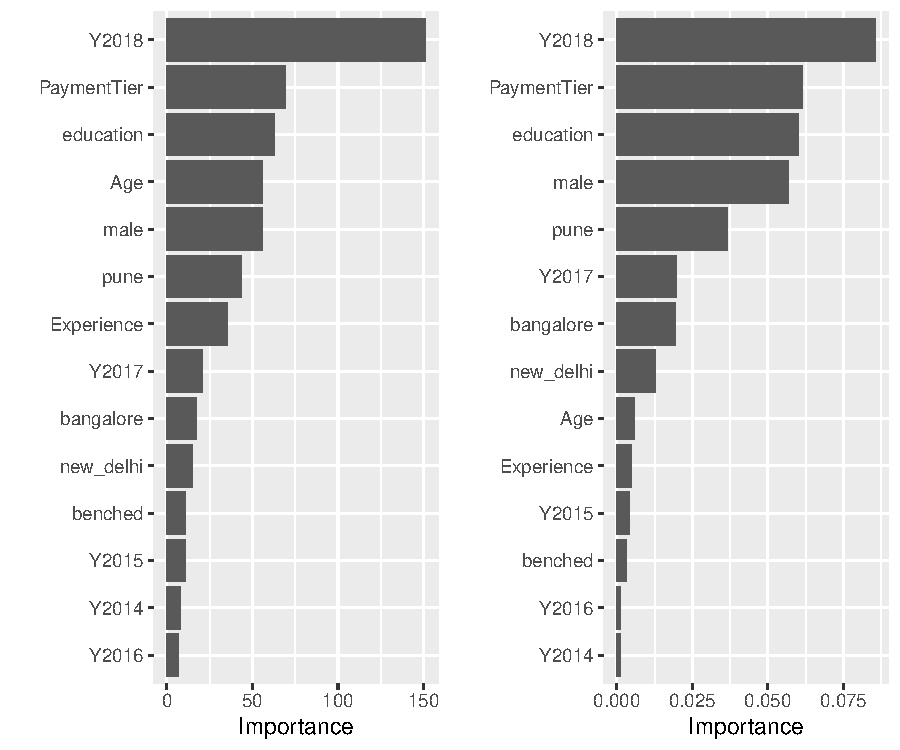
\includegraphics{Final_project_files/figure-latex/unnamed-chunk-17-1.pdf}

\hfill

\hypertarget{conclusion}{%
\section{Conclusion}\label{conclusion}}

In order to predict employee attrition, various models and their
accuracy levels are assessed.

The best model in predicting is the random forest model after
hyperparameter tuning. This model achieves an accuracy rate of 86
percent.

When assessing the bias-variance tradeoff\ldots{}

To cite this package, simply type citation(``Texevier'') in Rstudio to
get the citation for Katzke (\protect\hyperlink{ref-Texevier}{2017})
(Note that uncited references in your bibtex file will not be included
in References).

\newpage

\hypertarget{references}{%
\section*{References}\label{references}}
\addcontentsline{toc}{section}{References}

\hypertarget{refs}{}
\begin{CSLReferences}{1}{0}
\leavevmode\vadjust pre{\hypertarget{ref-Texevier}{}}%
Katzke, N.F. 2017. \emph{{Texevier}: {P}ackage to create elsevier
templates for rmarkdown}. Stellenbosch, South Africa: Bureau for
Economic Research.

\end{CSLReferences}

\bibliography{Tex/ref}





\end{document}
